\documentclass[a4paper,11pt]{article}

\usepackage[margin=3cm]{geometry}
\usepackage{amsfonts}
\usepackage{amsmath}
\usepackage{amssymb}
\usepackage{graphicx}
\usepackage{subcaption}


\usepackage[utf8]{inputenc}
%\usepackage[cp1250]{inputenc}
\usepackage[polish]{babel}
\usepackage[T1]{fontenc}


%----------------------
\def\\{\hfill\break}


%----------------------
\title{Projekt Egzaminacyjny}
\author{Maria Koren}
\date{Listopad 2023 - Styczeń 2024}

\begin{document}
\maketitle
\newpage
\tableofcontents{}
\newpage

\section{Wstęp}
W tym projekcie reprezentowana jest analiza danych spółek KMR.UK (Kenmare Resources Plc) oraz JJB (Jujubee S.A). 

Kenmare Resources plc to uznana firma wydobywcza, która zarządza kopalnią minerałów tytanu Moma położoną na północno-wschodnim wybrzeżu Mozambiku.
Kopalnia prowadzi produkcję komercyjną od 2009 roku i jest uznawana za głównego dostawcę produktów z piasku mineralnego dla klientów na całym świecie, działających w ponad
15 krajach.

Jujubee S.A. to studio deweloperskie zajmujące
się tworzeniem gier wideo, które ma swoim koncie
takie tytuły jak: „FLASHOUT 3D”, „Suspect in
Sight”, „Take Off – The Flight Simulator”,
strategię czasu rzeczywistego „Realpolitiks”, grę
przygodowo-dokumentalną „KURSK” oraz „Deep Diving
Simulator”. Studio zostało założone przez byłych
pracowników CD Projekt RED, Traveller’s Tales oraz
Inifinite Dreams. Celem firmy jest tworzenie niesamowicie
grywalnych i doskonale wyglądających gier na wszystkie
istotne platformy sprzętowe, takie jak iOS (iPhone,
iPod, iPad), Android, Mac, PC i konsole. Jujubee jest
spółką notowaną na rynku NewConnect (JJB).

W pierwszej części projektu analizowano kursy zamknięcia spółki KMR za 2022 rok. Badano jakie ma rozkłady za pomocą wykresów diagnostycznych oraz statystyk opisowych. W drugiej części projektu badano zależność międzu log-zwrotami kursów powyższych spółek. W trzeciej części projektu zrobiona regresja liniowa dla log-zwrotów

\newpage
\section{Analiza cen spółek}
\subsection{Analiza cen spółki KMR.UK}
\subsubsection{Wykres kursów zamknięcia pokazujący zmiany w czasie oraz
histogram}

Zrobiono wykres  kursu zamknięcia pokazujący zmiany w czasie, rysunek \ref{fig:cena_podcaz_zamkn}

\begin{figure}[h]
  \centering
  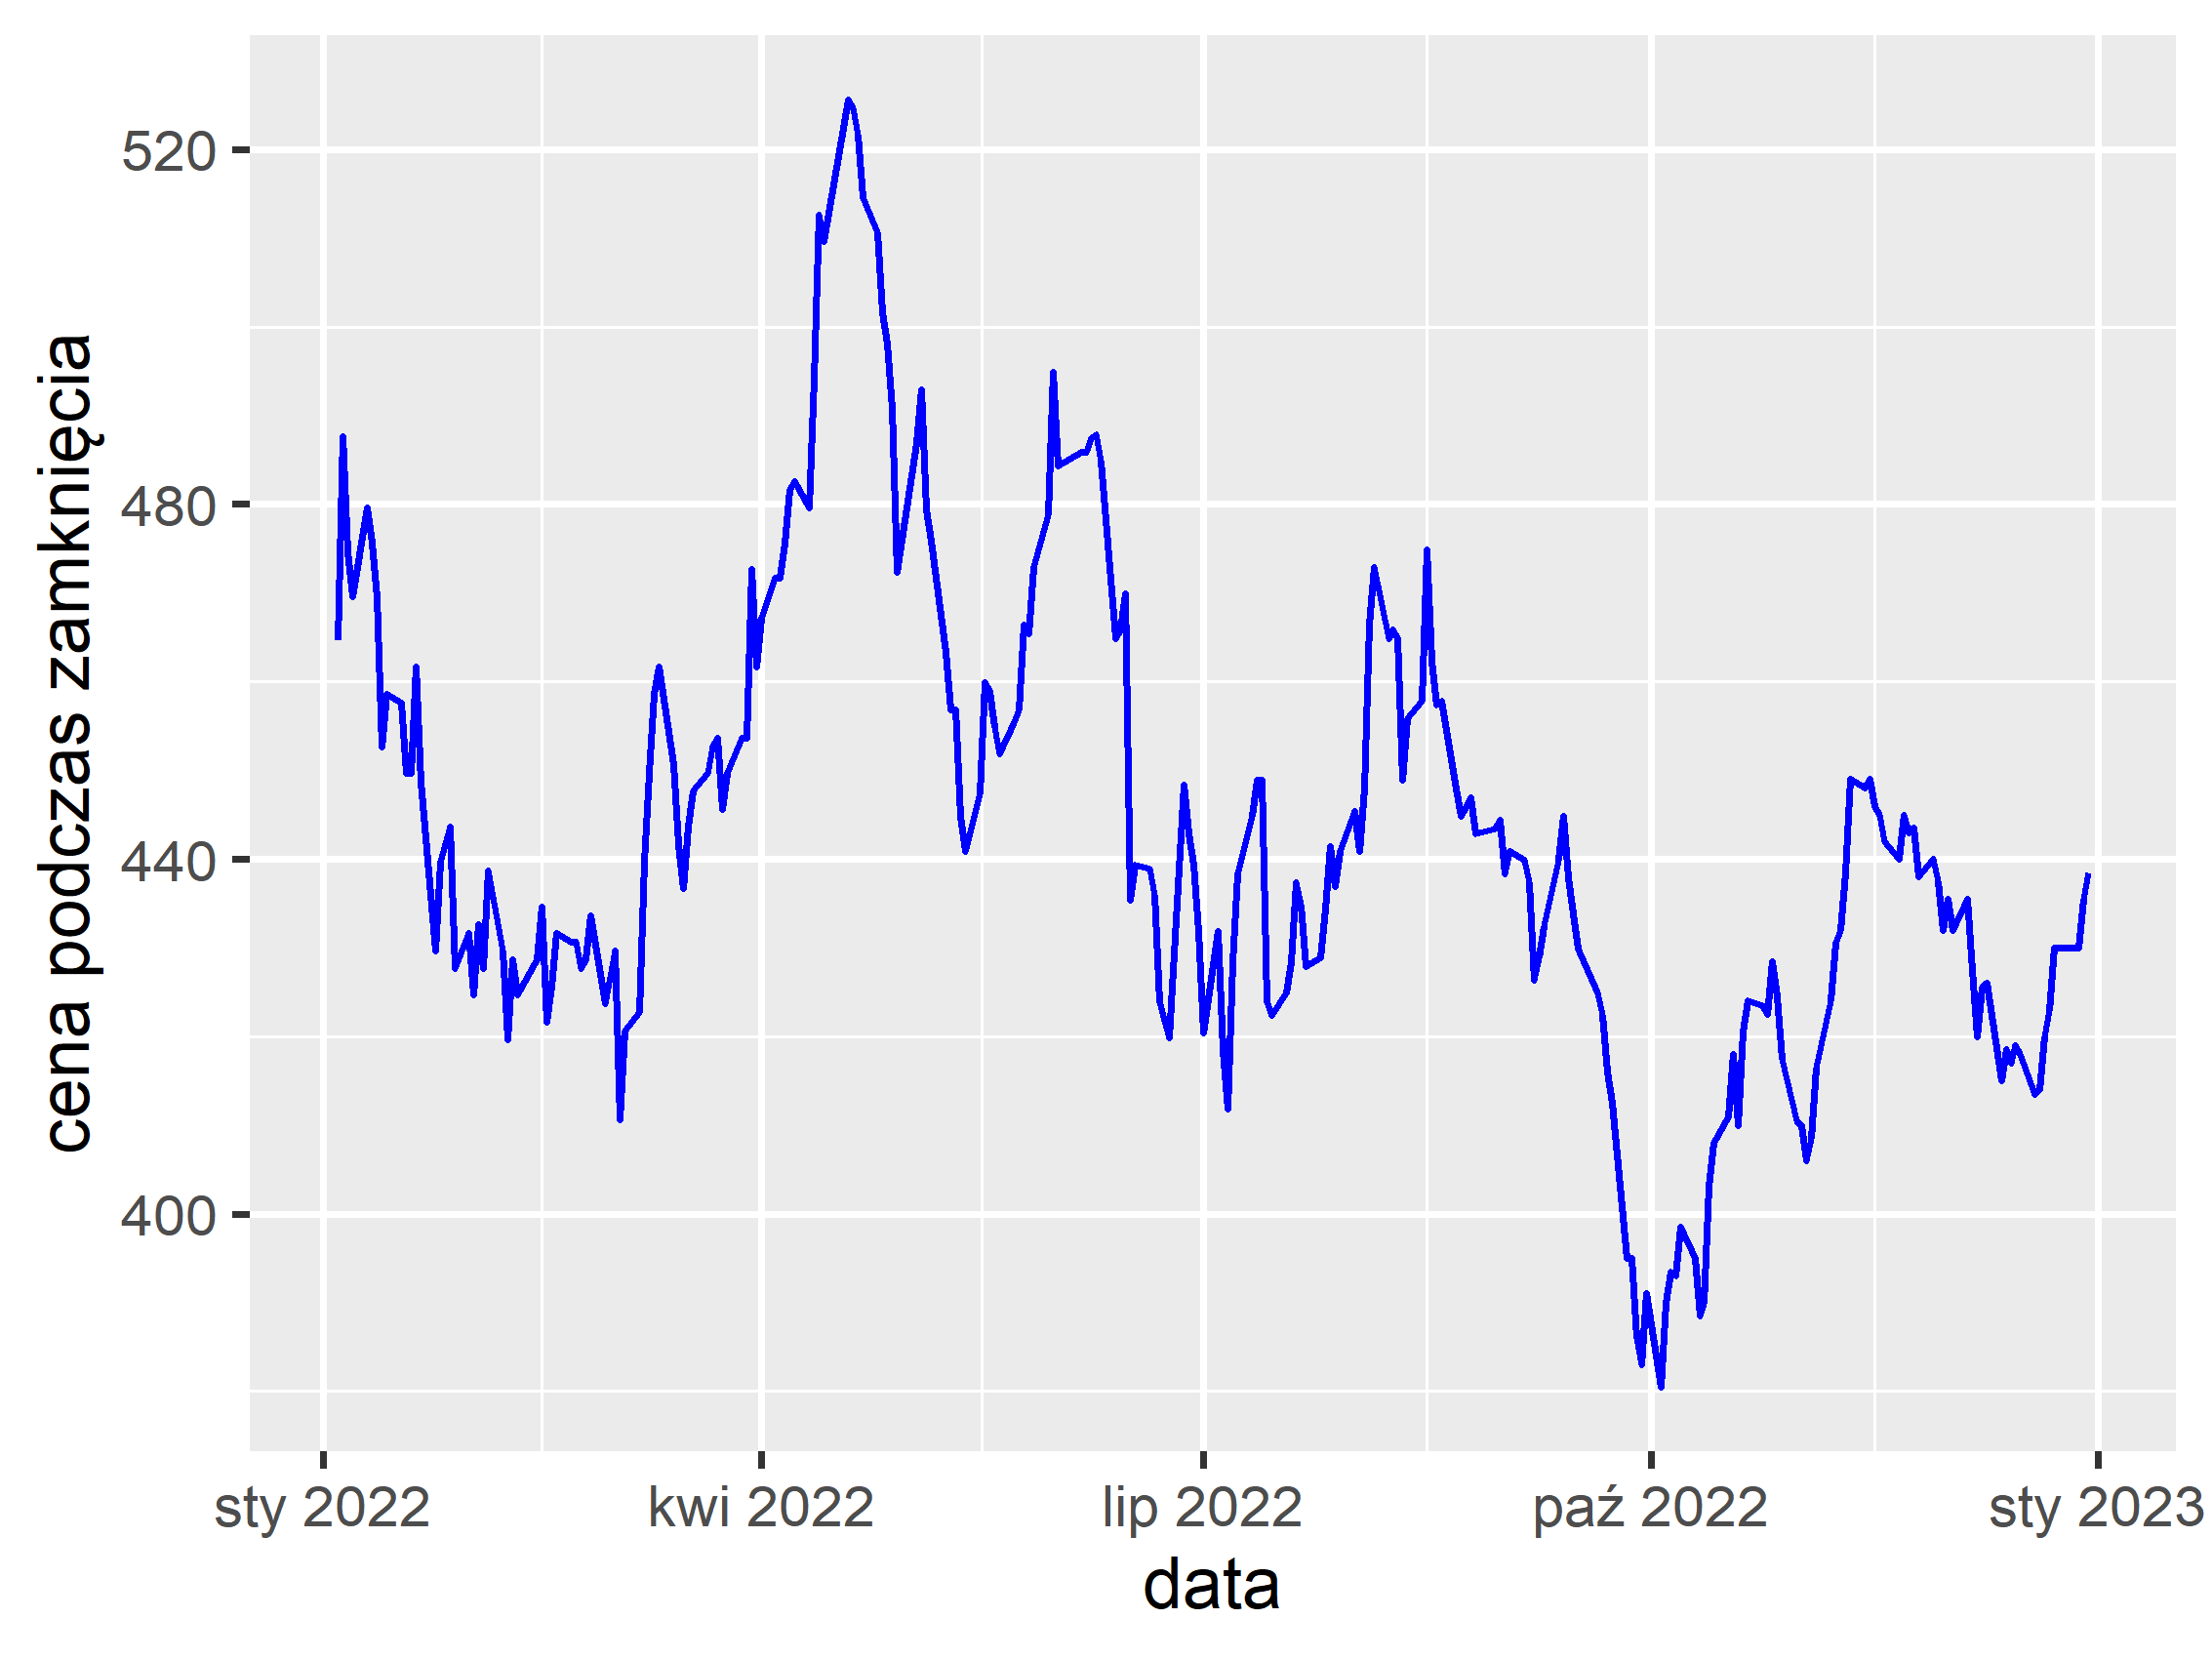
\includegraphics[width=10cm]{images/cena_poczas_zamkn.png}
  \caption{Cena podczas zamknięcia}
  \label{fig:cena_podcaz_zamkn}
\end{figure}

Oraz histogram, pokazujacy liczebność danych, rysunek \ref{fig:histogram}
\begin{figure}[h]
  \centering
  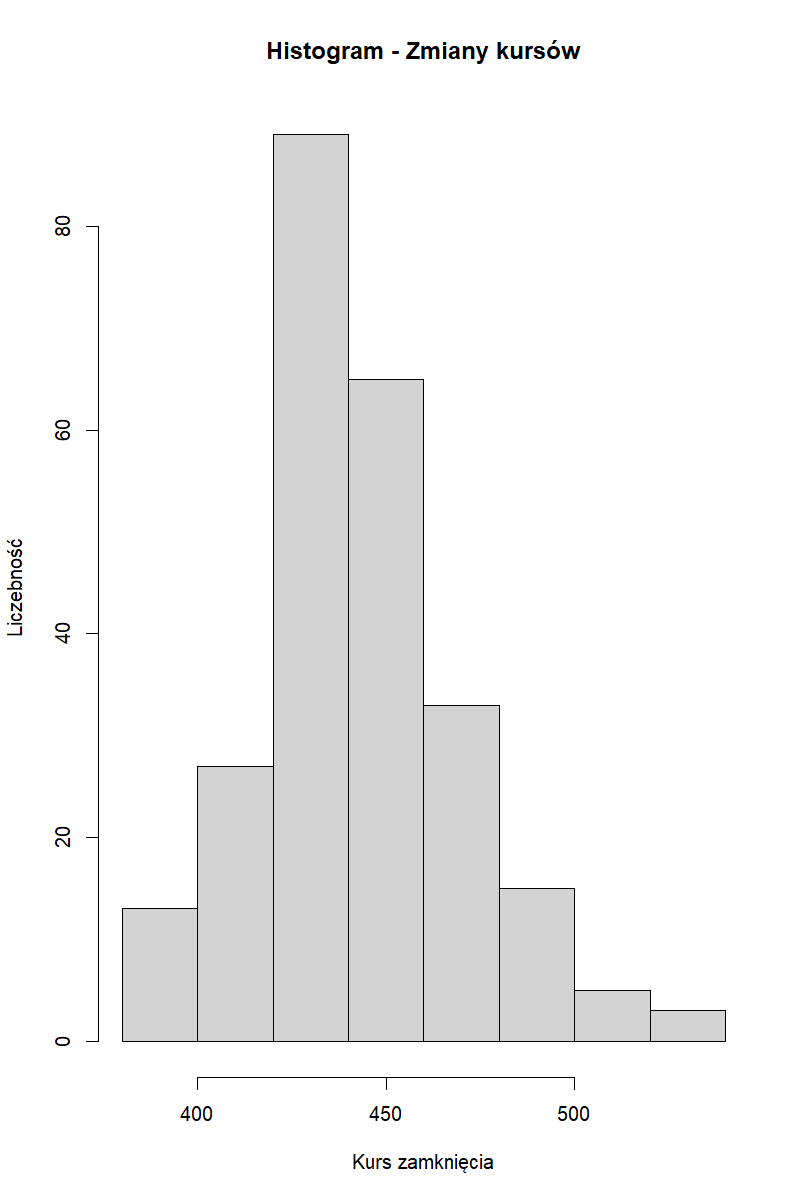
\includegraphics[width=10cm]{images/histogram.png}
  \caption{Histogram danych}
  \label{fig:histogram}
\end{figure}

\newpage
\subsubsection{Statystyki opisowe}

Zostały obliczone nastepujące statystyki opisowe: średnia, odchylenie standardowe, skośność oraz kurtoza

Wyniki statystyk znajdują się w poniższej tabeli \ref{tab:statystyki_opisowe}

\begin{table}[h]
  \centering
  \begin{tabular}{|c|c|c|c|c|}
    \hline
     & $\bar{x}$ & odch. st. & skośność & kurtoza  \\
    \hline
    akcje & 442.8741 & 26.7262 & 3.574323 & 0.52783 \\
    \hline

    \hline
  \end{tabular}
  \caption{Statystyki opisowe}
  \label{tab:statystyki_opisowe}
\end{table}

\paragraph{Interpretacja wyników}
\begin{itemize}
  \item Otrzymana skośność mówi o przewadzę wartości wyższych (wartość skośności powyżej zera)
  \item  Otrzymana kurtoza mówi cieńszych ogonach niż rozkład normalny (bardziej płaski) (wartość kurtozy mniej niż 3)

\end{itemize}


\subsubsection{Estymacja parametrów trzech rozkładów korzystając z estymatora największej wiarygodności (MLE)}

Wyestymowano wyniki trzech rozkładów: normalnego, log-normalnego oraz rozkładu Weibulla za pomocą estymatora MLE. Wyżej wymienione wykresy dodano do wcześniejszego histogramu, co widać za rysynku \ref{fig:histogram_wykresy}


\begin{figure}[h]
  \centering
  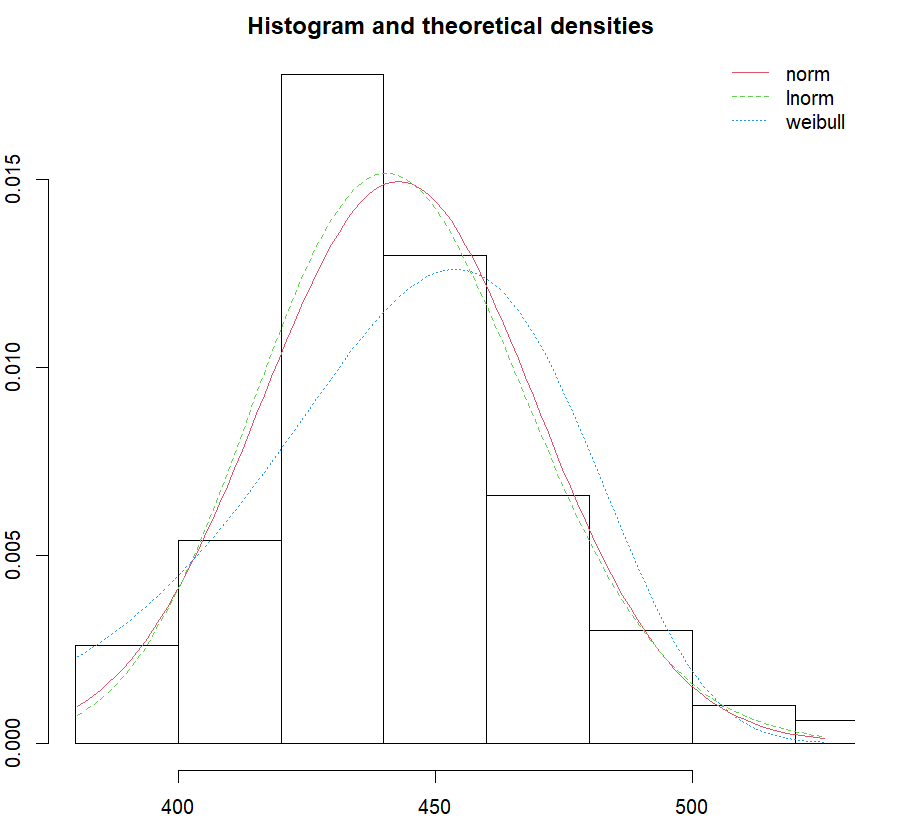
\includegraphics[width=10cm]{images/histogram_z_wykresami.png}
  \caption{Histogram wraz z estymowanami rozkładami}
  \label{fig:histogram_wykresy}
\end{figure}

Wyniki estymacji parametrów są przedstawione w tabeli \ref{wyniki_estymacji}
\begin{table}[h]
  \centering
  \begin{tabular}{|c|c|c|}
    \hline
     & $\mu$ & $\sigma$   \\
    \hline
    normalny & 442.8741 & 26.67269  \\
    \hline

    \hline
     & $\mu$ & $\sigma$   \\
    \hline
    log-normalny & 6.091499 & 0.05957788  \\
    \hline

    \hline
     & $a$ & $\sigma$   \\
    \hline
    weibulla & 15.61307 & 455.8914  \\
    \hline
  \end{tabular}
  \caption{Wyniki estymacji parametrów}
  \label{wyniki_estymacji}

\end{table}



Te wyniki oznaczają, że zostały dopasowane następujące rozkłady:

\begin{itemize}
  \item $X \sim\ N(442.87, 26.67)$
  \item $X \sim\ LN(6.09, 0.059)$
  \item $X \sim\ W(15.61, 455.89)$

\end{itemize}

\subsubsection{Wykresy diagnostyczne}
Zostały zrobione wykresy diagnostyczne qq-plot (rysunek \ref{fig:qqplot}) oraz cdf (rysunek \ref{fig:cdf})

\begin{figure}[!htb]
  \centering
  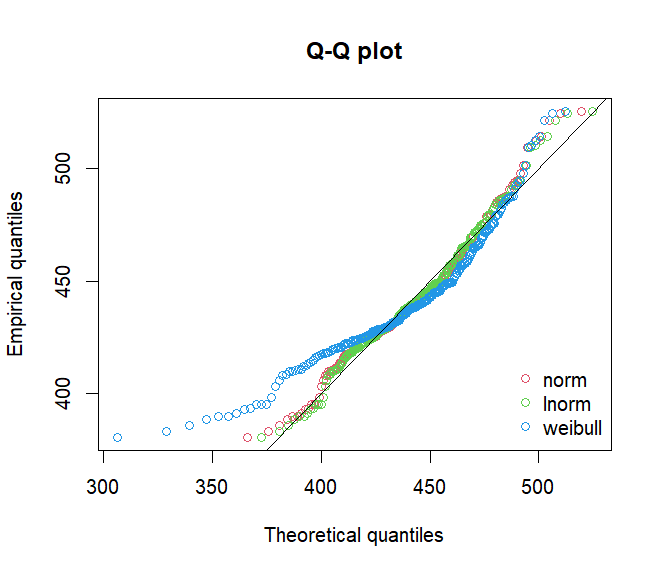
\includegraphics[width=9cm]{images/qqplot.png}
  \caption{Wykres qq-plot}
  \label{fig:qqplot}
\end{figure}

\begin{figure}[!htb]
  \centering
  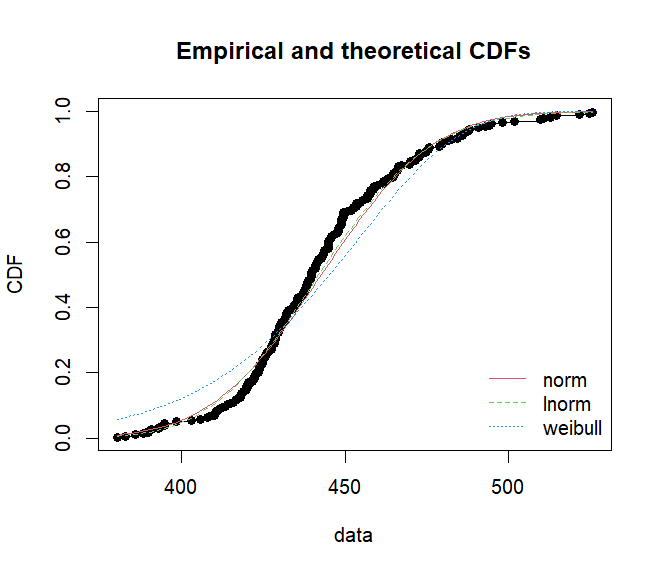
\includegraphics[width=9cm]{images/cdf.png}
  \caption{Wykres cdf}
  \label{fig:cdf}
\end{figure}

\begin{itemize}
  \item Wykres qq-plot
  
 Jest to wykres kwantyl-kwantyl, na osi pionowej są kwantyle teoretyczne, na osi   poziomowej są kwantyle empiryczne. Kwantyl rzędu $\alpha$  $\in$ (0, 1) zmiennej losowej ciągłej $X$ to taka liczba q, dla której prawdopodobieństwo, że zmienna $X$ przyjmuje   wartości mniejsze lub równe q jest równe $\alpha$.
      
  Najlepiej jest gdy te kwantyle są takie same bądź bardzo blizkie siebie. Dlatego   najlepszym rozkładem  jest najbliższy do prostej $y=x$. W rozważanym przykład takim   jest wykres log-normalny $X \sim\ LN(6.09, 0.059)$
  \item Wykres CDF

  Funkcja rozkładu kumulacyjnego (CDF, Cumulative Distribution Function) to graficzna reprezentacja kumulatywnej dystrybuanty danej zmiennej losowej. CDF dla danej wartości $x$ to prawdopodobieństwo, że zmienna losowa przyjmuje wartość mniejszą lub równą $x$. Czarnym zaznaczone są dane empiryczne. Najlepszym wykresem jest mający teorytyczne dane najbliższe do danych empirycznych. W rozważanym przykładzie takim wykresem jest log-normalny $X \sim\ LN(6.091, 0.059)$
\end{itemize}

Na podstawie wykresów diagnostycznych najlepszym rozkładem jest rozkład logarytmiczno-normalny

\paragraph{Analiza wartości statystyk KS, CM i AD oraz kryteria informacyjne AIC i BIC}
\\
Bazując wyłącznie na wykresach diagnostycznych, nie jest możliwe wybranie najlepszego wykresu. Dlatego skorzystano ze statystyk Kołmogorowa-Smirnowa, Cramera-von-Misesa, Andersona-Darlinga, a także z kryteriów informacyjnych AIC (Akaike's Information Criterion) oraz BIC (Bayesian Information Criterion)

Wartości ze statystyk KS, CM, AD są umieszczone w tabeli \ref{tab:statystyki}. Wartości kryteriów AIC, BIC w tabeli \ref{tab:kryteriaInf}


\begin{table}[!htb]
  \centering
  \begin{tabular}{|c|c|c|c|}
    \hline
     & normalny & log-normalny & weibull  \\
    \hline
    Kolmogorov-Smirnov & 0.09168955 & 0.0798396 & 0.138442\\
    \hline
    Cramer-von Mises & 0.3613063 & 0.2485924 & 1.257677 \\
    \hline
    Anderson-Darling & 2.005469 & 1.412547 & 7.416593 \\
    \hline
  \end{tabular}
  \caption{Statystyki}
  \label{tab:statystyki}
\end{table}


\begin{table}[!htb]
  \centering
  \begin{tabular}{|c|c|c|c|}
    \hline
     & normalny & log-normalny & weibull  \\
    \hline
    Akaike's Information Criterion & 2355.289 & 2348.983 & 2415.692\\
    \hline
    Bayesian Information Criterion & 2362.332 & 2356.026 & 2422.735 \\
    \hline
  \end{tabular}
  \caption{Kryteria informacyjne}
  \label{tab:kryteriaInf}
\end{table}

Ponieważ statystyki są oparte na porównaniu odległości dystrybuant, najlepszym rozkładem jest ten, który jest najbliżej do danych teorytycznych (ma najmniejszą odległość), czyli ma najmniejszą wartość statystyki. W kryteriach informacyjnych za najlepszy rozkład również jest uważany rozkład, mający najmniejszą wartosć kryteria. W rozważanym przykładzie takim rozkładem jest rozkład log-normalny $X \sim\ LN(6.09, 0.059)$

\subsubsection{Testowanie hipotezy o równości rozkładów, wykorzystując  statystykę KS}

Zrobiona hipoteza H0: $F=LN(6.09, 0.0595)$ przeciwko hipotezie H1: F nie jest rowny $LN(6.09, 0.059)$

Zgenerowano $N=10000$ probek licznosci $n$ (równej ilości danych) z rozkładu $F0=LN(6.09, 0.059)$ wybranego wcześniej jako najlepszego rozkładu i obliczono odleglość dystrybuant empirycznych od rozkladu F0 (wartosc statystyki Dn)

Obliczona również wartość statystyki dla rzeczywustych danych

Rysowany jest histogram statystyk testu KS uzyskanych z danych losowych, a także dodany jest punkt dla statystyki testu KS uzyskanej z rzeczywistych danych dla porównania danych rzeczywistych z danymi losowymi tego rozkładu


\begin{figure}[!htb]
  \centering
  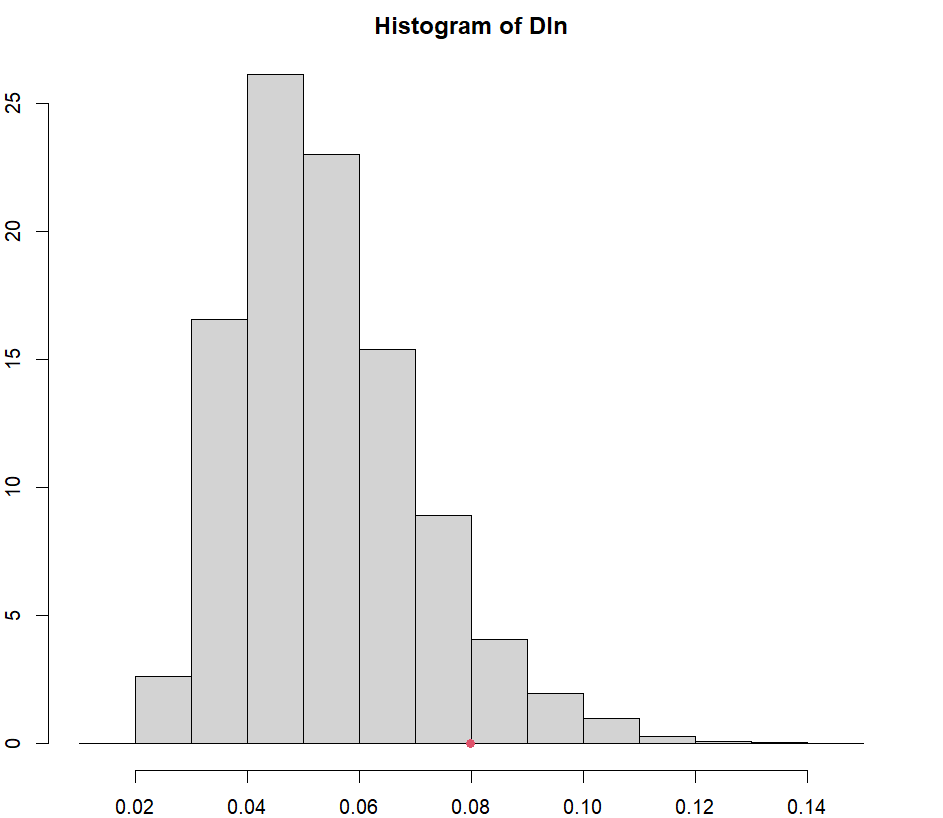
\includegraphics[width=9cm]{images/histogram_dane_teoryteczne.png}
  \caption{Histogram danych teorytycznych}
  \label{fig:hisT_dane_teor}
\end{figure}

Z wykresu widać, że wynik z danych rzeczywistych jest umieszczony w miejscu, gdzie dane losowe jeszcze są



Ta statystyka zwraca 2 informacje: odległość (wartość \textit{statistic}) oraz prawdopodobieństwo że wartości statystyki KS są takie same lub większe, gdy hipoteza zerowa jest prawdziwa

Wyniki tego testowania zostaną umieszczone w tabeli \ref{tab:wyniki_testowania}:

\begin{table}[!htb]
  \centering
  \begin{tabular}{|c|c|}
    \hline
     statistic & p-value   \\
    \hline
     0.0798396  & 0.0827\\
    \hline
  \end{tabular}
  \caption{Wartość statystyki KS w testowaniu hipotezy}
  \label{tab:wyniki_testowania}
\end{table}


P-wartość informuje o prawdopodobieństwie uzyskania takiej samej lub bardziej ekstremalnej statystyki testu, niż ta, którą otrzymaliśmy z danych rzeczywistych (zakładając że dane pochodzą z tego samego rozkładu)

Ponieważ p-wartosć  $p = 0.0827 > 0.05$ zatem nie ma powodów odrzucenia hipotezy. Uzyskane wyniki potwierdzają wybraną hipotezę  o logarytmiczno-normalnym $LN(6.09, 0.059)$ rozkładzie danych

\newpage

\pagebreak
\section{Analiza łącznego rozkładu log-zwrotów}
\subsection{Analiza rozkładów brzegowych}
\subsubsection{Analiza rozkładów brzegowych spółki KMR}

Na rysynkach \ref{fig:kmr_wykres_log} oraz \ref{fig:kmr_hist_log} są przedstawione odpowiednio wykresy log-zwrotów oraz histogram
\begin{figure}[!htb]
    \centering

    \begin{minipage}{.45\textwidth}
        \centering
        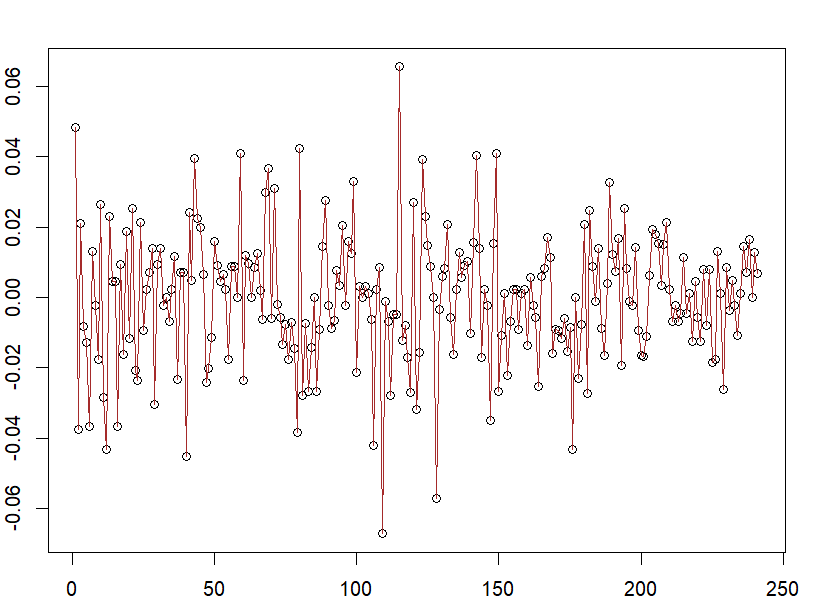
\includegraphics[width=\linewidth]{images/kmr_wykres_log.png}
        \caption{Wykres log-zwrotów spółki KMR}
        \label{fig:kmr_wykres_log}
    \end{minipage}\hspace{0.1\textwidth}% Adjust the space here
    \begin{minipage}{.45\textwidth}
        \centering
        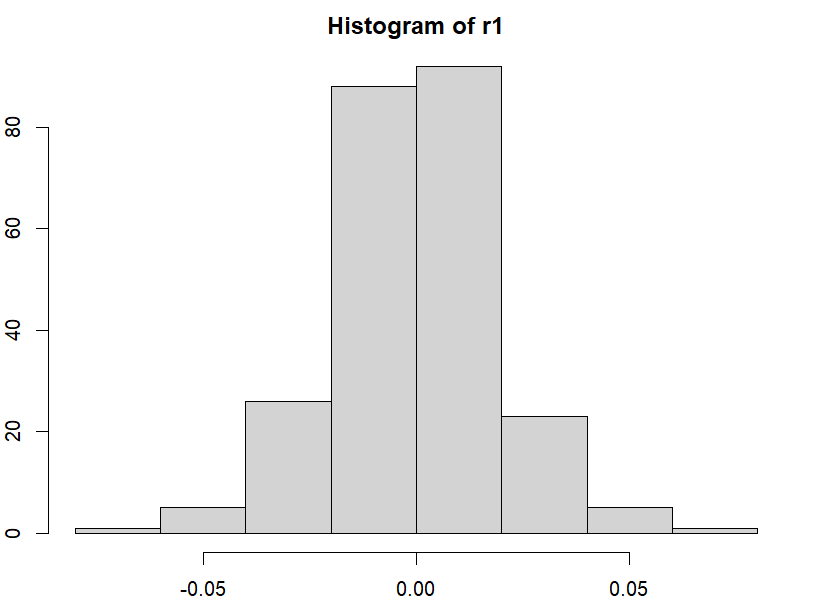
\includegraphics[width=\linewidth]{images/kmr_hist_log.png}
        \caption{Wykres log-zwrotów spółki KMR}
        \label{fig:kmr_hist_log}
    \end{minipage}
\end{figure}

Został dopasowany do tych danych rozkład normalny $X \sim\ N(-0.0023, 0.018)$, rysunek \ref{fig:kmr_histwykres_log}

\begin{figure}[!htb]
    \begin{minipage}{0.45\textwidth}
        \centering
        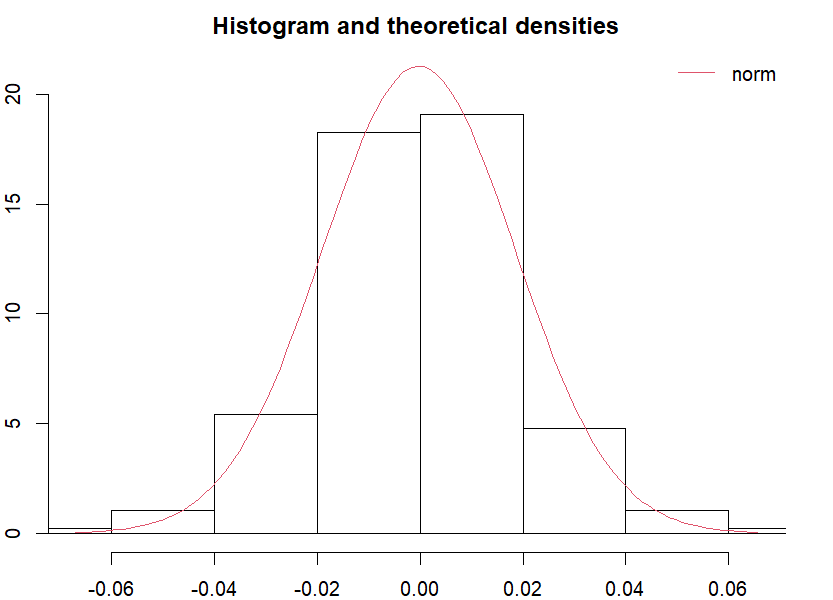
\includegraphics[width=\linewidth]{images/kmr_histW_log.png}
        \caption{Wykres log-zwrotów wraz z dopasowanym rozkładem normalnym spółki KMR}
        \label{fig:kmr_histwykres_log}
    \end{minipage}\hspace{0.05\textwidth}%
    \begin{minipage}{0.45\textwidth}
        \centering
        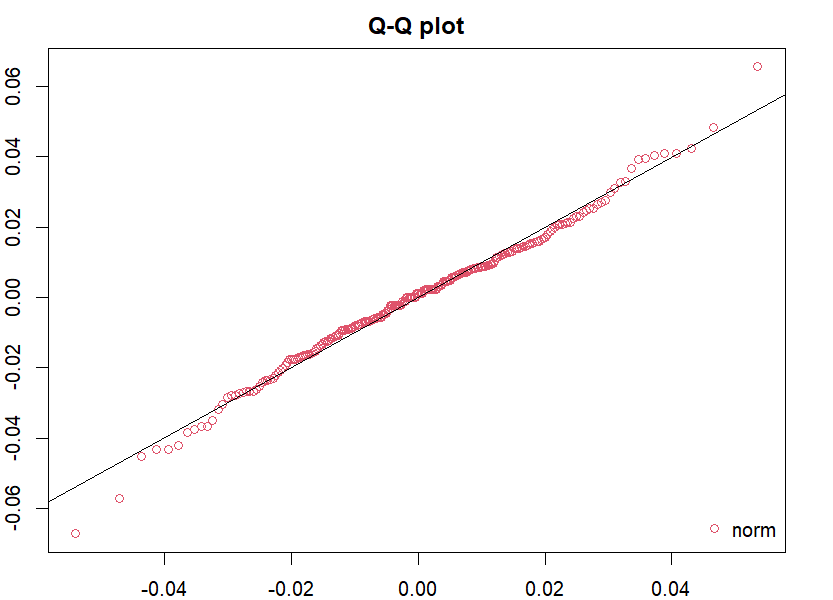
\includegraphics[width=\linewidth]{images/kmr_qqplot_log.png}
        \caption{Wykres qqplot dla log-zwrotów spółki KMR}
        \label{fig:kmr_qqplot_log}
    \end{minipage}

    \begin{minipage}{0.45\textwidth}
        \centering
        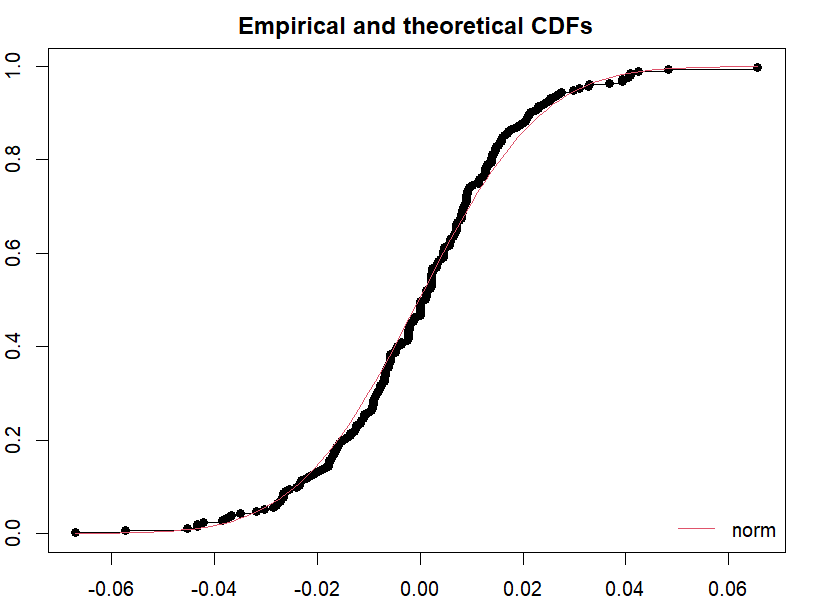
\includegraphics[width=\linewidth]{images/kmr_cdf_log.png}
        \caption{Wykres cdf dla log-zwrotów spółki KMR}
        \label{fig:kmr_cdf_log}
    \end{minipage}\hspace{0.05\textwidth}%
    \begin{minipage}{0.45\textwidth}
        \centering
        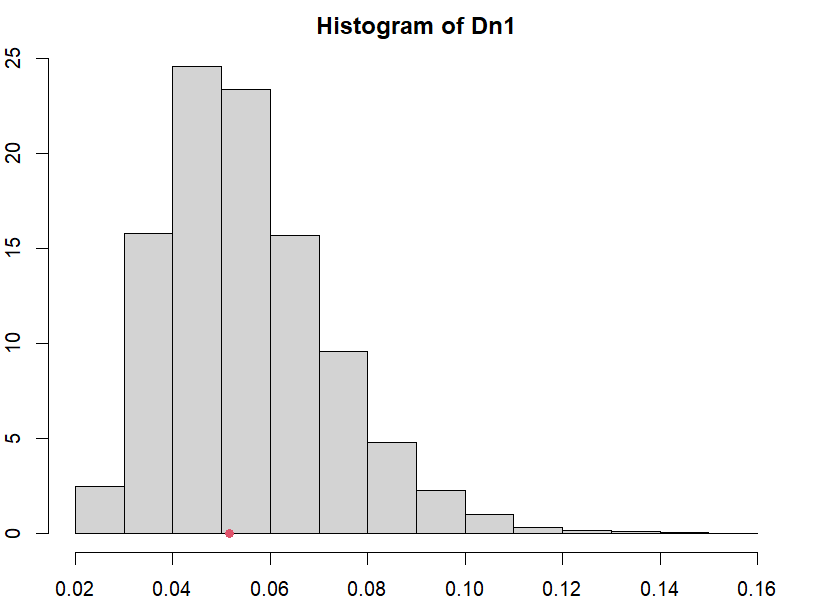
\includegraphics[width=\linewidth]{images/kmr_histMC.png}
        \caption{Histogram danych w teście}
        \label{fig:kmr_histMC}
    \end{minipage}
\end{figure}

Zrobiono wykresy diagnostyczne cdf oraz qqplot, rysunki \ref{fig:kmr_qqplot_log}, \ref{fig:kmr_cdf_log}



Przeprowadzono również test równości metodą Monte-Carlo. Skorzystano ze statystyki Kolmogorova-Smirnova. Wynik p-value otrzymany w tym teście jest równy 0.5656, co oznacza brak podstaw do odrzucenia hipotezy że rozklad log-zwrotów jest  $X \sim\ N(-0.0023, 0.018)$, rysunek \ref{fig:kmr_histMC}



\subsubsection{Analiza rozkładów brzegowych spółki JJB}

Na rysynkach \ref{fig:jjb_wykres_log} oraz \ref{fig:jjb_hist_log} są przedstawione odpowiednio wykresy log-zwrotów oraz histogram
\begin{figure}[!htb]
    \centering

    \begin{minipage}{.45\textwidth}
        \centering
        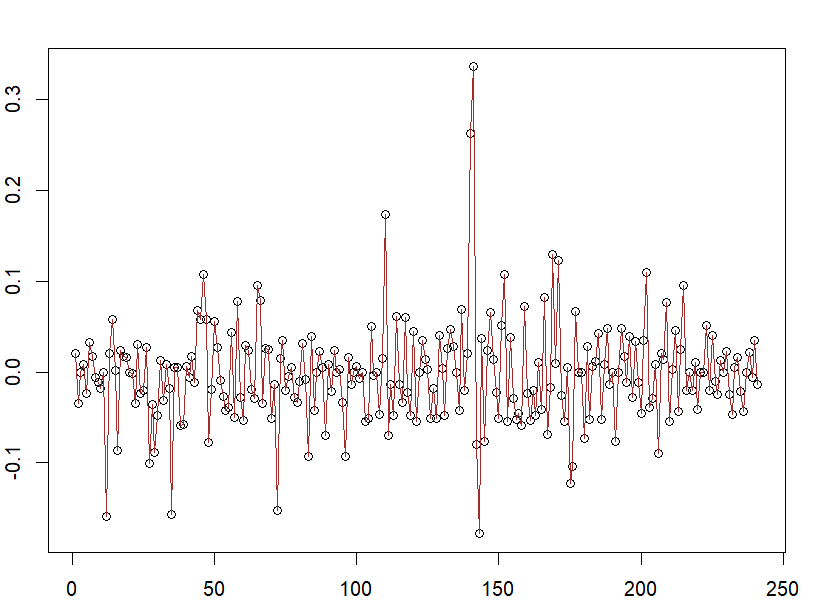
\includegraphics[width=\linewidth]{images/jjb_wykres_log.png}
        \caption{Wykres log-zwrotów spółki JJB}
        \label{fig:jjb_wykres_log}
    \end{minipage}\hspace{0.1\textwidth}% Adjust the space here
    \begin{minipage}{.45\textwidth}
        \centering
        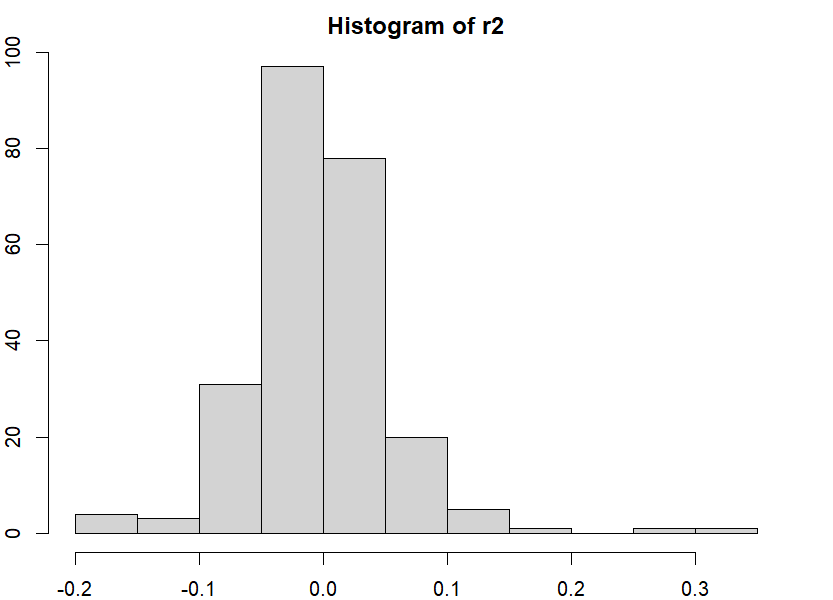
\includegraphics[width=\linewidth]{images/jjb_hist_log.png}
        \caption{Wykres log-zwrotów spółki JJB}
        \label{fig:jjb_hist_log}
    \end{minipage}
\end{figure}

Został dopasowany do tych danych rozkład normalny $Y \sim\ N(-0.0025,0.057 )$, rysunek \ref{fig:jjb_histwykres_log}




Zrobiono wykresy diagnostyczne cdf oraz qqplot, rysunki \ref{fig:jjb_qqplot_log}, \ref{fig:jjb_cdf_log}

Przeprowadzono również test równości metodą Monte-Carlo. Skorzystano ze statystyki Kolmogorova-Smirnova. Wynik p-value otrzymany w tym teście jest równy 0.5709, co nie daje powodów do odrzucenia hipotezy że rozklad log-zwrotów jest  $Y \sim\  N(-0.0025,0.057 )$

\subsection{Estymacja parametrów rozkładu dwuwymiarowego normalnego oraz analiza dobroci dopasowania}

\subsubsection{Wykres rozrzutu z histogramami rozkładów brzegowych}

Zrobiono wykres rozrzutu z histogramami brzegowymi, rysunek \ref{fig:wykres_rozrzutu}. Wykres rozrzutu wizualizuje zależności między dwiema zmiennymi. Każdy punkt na wykresie reprezentuje log-zwroty spółek jednego dnia. Rozproszenie danych na podanym wykresie sugeruje że log-zwroty rozważanych spółek mogą mieć rozkład dwuwymiarowy normalny

\begin{figure}[!htb]
    \begin{minipage}{0.48\textwidth}
        \centering
        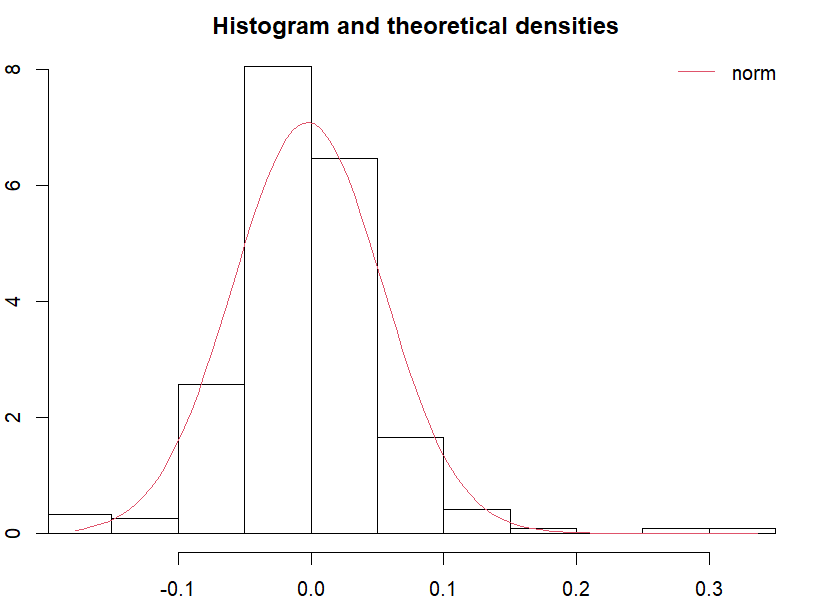
\includegraphics[width=\linewidth]{images/jjb_histwykres_log.png}
        \caption{Wykres log-zwrotów wraz z dopasowanym rozkładem normalnym spółki JJB}
        \label{fig:jjb_histwykres_log}
    \end{minipage}\hfill
    \begin{minipage}{0.48\textwidth}
        \centering
        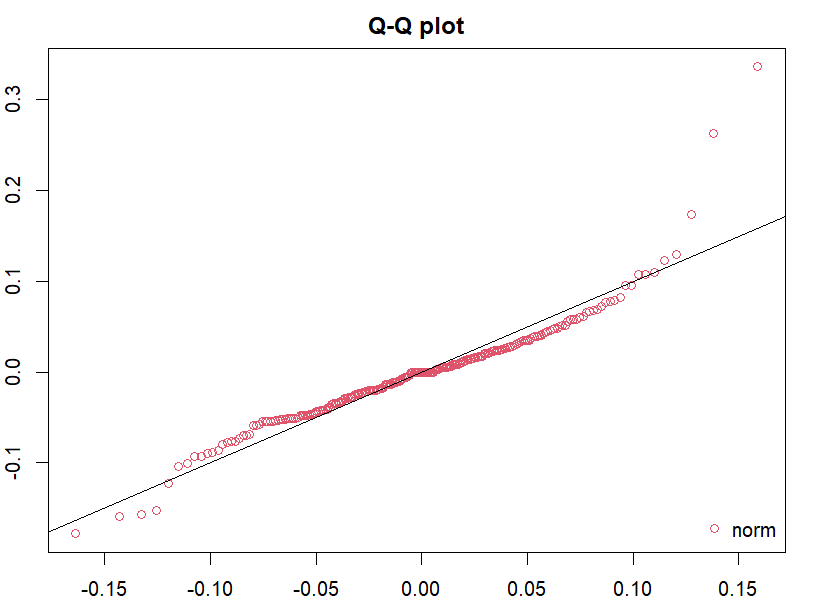
\includegraphics[width=\linewidth]{images/jjb_qqplot_log.png}
        \caption{Wykres qqplot dla log-zwrotów spółki JJB}
        \label{fig:jjb_qqplot_log}
    \end{minipage}
    \vspace{\baselineskip}
    \begin{minipage}{0.48\textwidth}
        \centering
        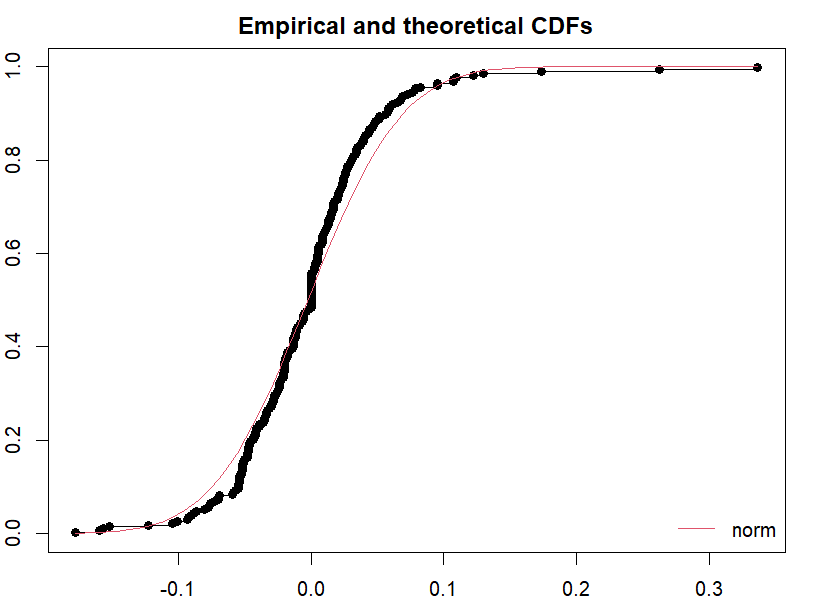
\includegraphics[width=\linewidth]{images/jjb_cdf_log.png}
        \caption{Wykres cdf dla log-zwrotów spółki JJB}
        \label{fig:jjb_cdf_log}
    \end{minipage}\hfill
    \begin{minipage}{0.48\textwidth}
        \centering
        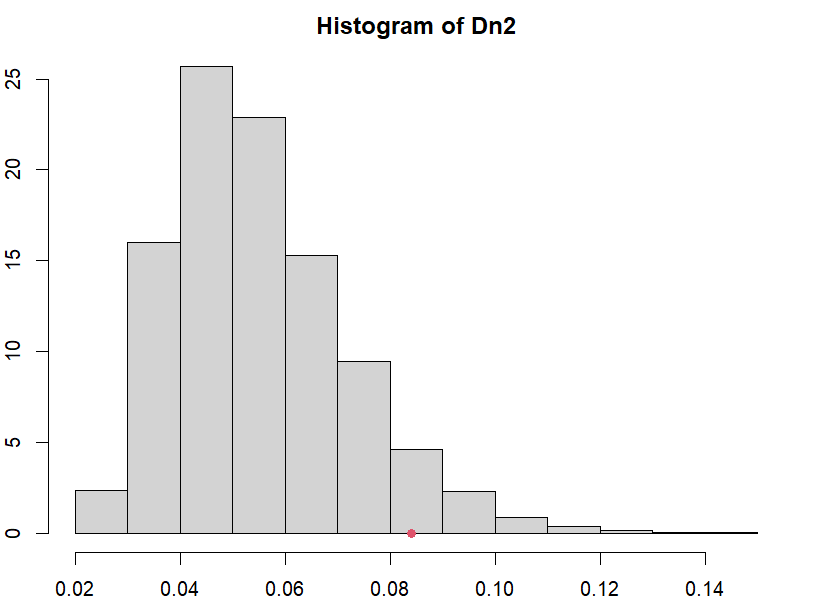
\includegraphics[width=\linewidth]{images/jjb_histMC.png}
        \caption{Histogram danych w teście}
        \label{fig:jjb_histMC}
    \end{minipage}

\end{figure}

\begin{figure}[!htb]
	\centering
	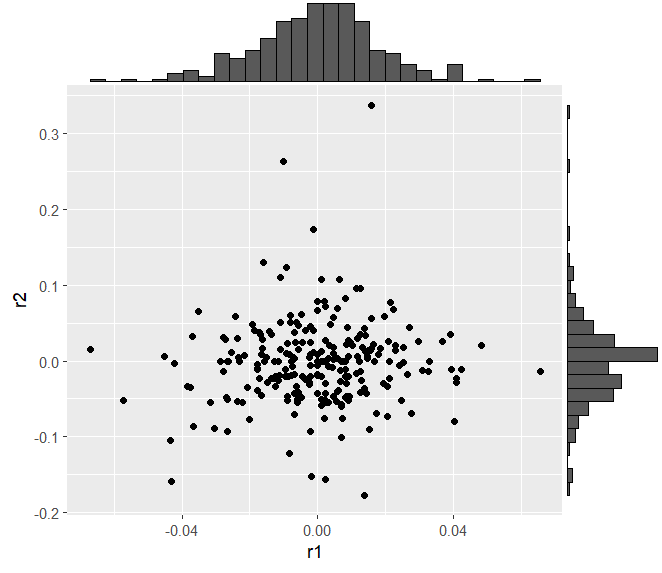
\includegraphics[width=8cm]{images/wykres_rozrzutu_histogram.png}
	\caption{Wykres rozrzutu z histogramami brzegowymi}
         \label{fig:wykres_rozrzutu}
\end{figure}


\subsubsection{Wektor średnich, kowariancji, macierz korelacji, współczynnik korelacji}

Zostały obliczone następujące estymatory:
\\
Wektor średnich:

\begin{table}[!htb]
\centering
\begin{tabular}{|c|c|}
\hline
$\mu_1$ & $\mu_2$ \\
\hline
-0.0002403422 & -0.0024970847 \\
\hline
\end{tabular}
\caption{Wektor średnich }
\end{table}

Macierz kowariancji (tabela \ref{tab:macierz_kowariancji}), współczynnik kowariancji $cov(X, Y) = 7.719315e-05$

\begin{table}[!htb]
\centering
\begin{tabular}{|c|c|c|}
\hline
& $r_1$ & $r_2$ \\
\hline
$r_1$ &3.529462e-04 & 7.719315e-05 \\
\hline
$r_2$ & 7.719315e-05 & 3.181408e-03 \\
\hline
\end{tabular}
\caption{Macierz kowariancji }
\label{tab:macierz_kowariancji}
\end{table}

Macierz korelacji (tabela \ref{tab:macierz_korelacji}). Współczynnik korelacji przyjmuje wartości z przedziału $[-1; 1]$ i wskazuje na stopień zależności dwóch zmiennych, im bliżej wartości bezwzględnej 1, tym silniejszy związek. W tym przypadku $\rho = 0.0728$ wskazuje że log-zwroty rozważanych spółek są słabo-dodatnio skorelowane

\begin{table}[!htb]
\centering
\begin{tabular}{|c|c|c|}
\hline
& $r_1$ & $r_2$ \\
\hline
$r_1$ &1.00000000 & 0.07284753 \\
\hline
$r_2$ & 0.07284753 & 1.00000000 \\
\hline
\end{tabular}
\caption{Macierz korelacji }
\label{tab:macierz_korelacji}
\end{table}





\subsubsection{Wzór gęstości rozkładu dwuwymiarowego normalnego}

Wyestymowane wcześniej parametry oznaczają że do log-zwrotów spółek został dopasowany rozkład 
$$(X, Y) \sim\ N(-0.000240342, -0.0024970847, 0.01878686, 0.05640397, 0.0728)$$
Inaczej zapisując:
$$(X, Y) \sim\ N(\begin{bmatrix}
                -0.0002403 & -0.002497  \\
                \end{bmatrix}, \begin{bmatrix}
                                3.529462e-04 & 7.719315e-05 \\
                                7.719315e-05 & 3.181408e-03  \\
                                \end{bmatrix})$$

Gęstość dopasowanego rozkładu 
\begin{equation}
\begin{split}
f(x, y) = & \frac{1}{2\pi \cdot 0.01878686 \cdot 0.05640397 \cdot \sqrt{1-0.0728^2}} \\
& \exp\left(-\frac{1}{2(1-0.0728^2)}\left[\frac{(x+0.000240342)^2}{ 0.01878686^2} \right.\right. \\
& \left.\left.- 2 \cdot 0.0728\frac{(x+0.000240342)(y+0.0024970847)}{ 0.01878686 \cdot 0.05640397} + \frac{(y+0.0024970847)^2}{0.05640397^2}\right]\right)
\end{split}
\end{equation}


Rozkład brzegowy dla spółki KMR: $ X \sim\ N(-0.000240342, 0.01878686)$.
Gęstość rozkładu brzegowego:
\begin{equation}
    f(x) = \frac{1}{\sqrt{2\pi}\cdot0.01878686} \exp\left(-\frac{1}{2}\left(\frac{x + 0.000240342}{0.01878686}\right)^2\right)
\end{equation}


Rozkład brzegowy dla spółki JJB: $ Y \sim\ N(-0.0024970847,0.05640397)$.
Gęstość rozkładu brzegowego:
\begin{equation}
    f(y) = \frac{1}{\sqrt{2\pi}\cdot0.05640397} \exp\left(-\frac{1}{2}\left(\frac{y + 0.0024970847}{0.05640397}\right)^2\right)
\end{equation}

Wykres gęstości rozkładu łącznego (rysunek \ref{fig:wykres_laczny}):

\begin{figure}[!htb]
	\centering
	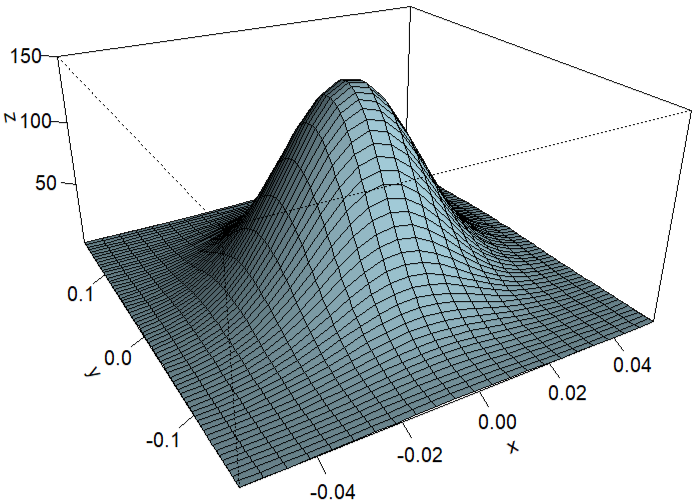
\includegraphics[width=8cm]{images/wykres3d.png}
	\caption{Wykres gęstości rozkładu łącznego }
         \label{fig:wykres_laczny}
\end{figure}

Wykres gęstości rozkładu brzegowego KMR (rysunek \ref{fig:wykres_gestosc_r1}).
Wykres gęstości rozkładu brzegowego JJB (rysunek \ref{fig:wykres_gestosc_r2})
\begin{figure}[!htb]
    \begin{subfigure}{0.45\textwidth}
        \centering
        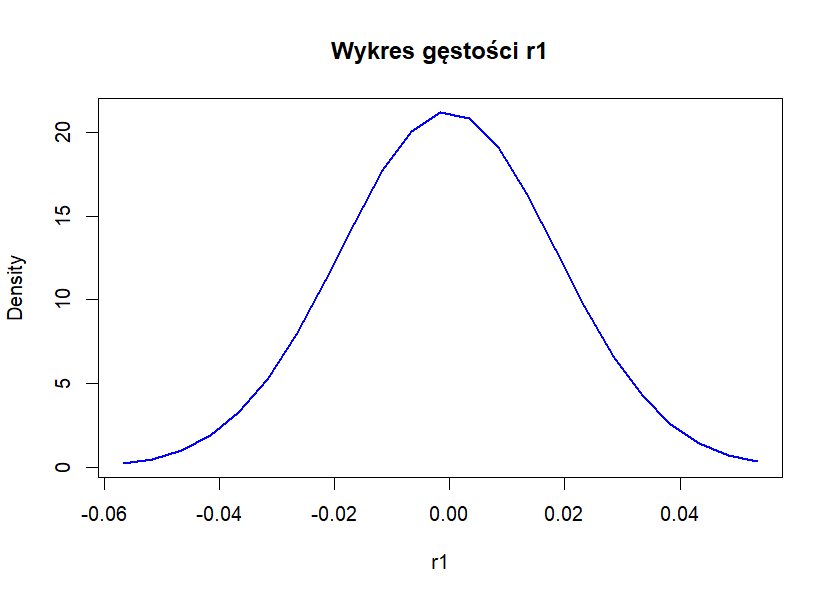
\includegraphics[width=\linewidth]{images/wykres_gestosc_r1.png}
        \caption{Wykres gęstości X}
        \label{fig:wykres_gestosc_r1}
    \end{subfigure}\hfill
    \begin{subfigure}{0.45\textwidth}
        \centering
        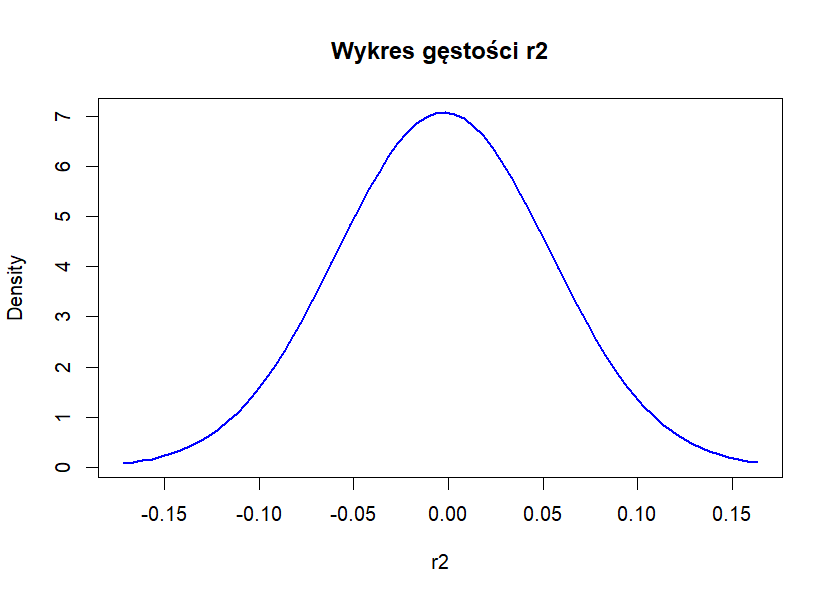
\includegraphics[width=\linewidth]{images/wykres_gestosc_r2.png}
        \caption{Wykres gęstości Y}
        \label{fig:wykres_gestosc_r2}
    \end{subfigure}
    
    \caption{Wykresy gęstości rozkładów brzegowych}
\end{figure}




\subsection{Analiza dopasowania rozkładu}
\subsubsection{Porównanie wykresów rozrzutu w oparciu o wygenerowaną próbę}
Z rozkładu $(X, Y) \sim\ N(-0.000240342, -0.0024970847, 0.01878686, 0.05640397, 0.0728)$ została wygenerowana próba liczności 241 (ponieważ taką liczność mają dane log-zwrotów spółek), rysunek \ref{fig:wykresy_rozrzutu}.
\begin{figure}[!htb]
	\centering
	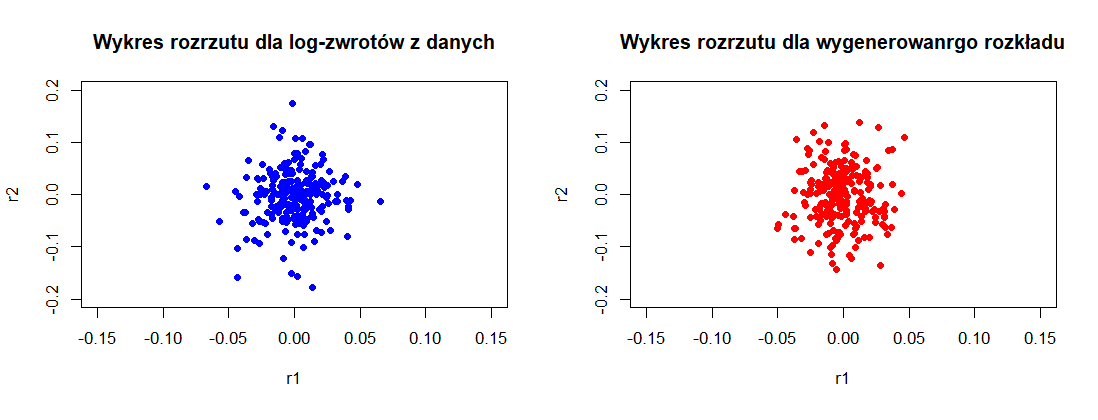
\includegraphics[width=10cm]{images/wykres_rozrzutu_porownanie.png}
	\caption{Wykresy rozrzutu wygenerowanej próby oraz danych }
         \label{fig:wykresy_rozrzutu}
\end{figure}
Analizując powyższe wykresy zauważano podobieństwo kształtów wykresu log-zwrotów rzeczywistych danych, oraz wykresu z wygenerowanego rozkładu. Na podstawie tego podobieństwa zrobiona hipoteza, że rozkład log-zwrotów może być $(X, Y) \sim\ N(-0.000240342, -0.0024970847, 0.01878686, 0.05640397, 0.0728)$ dobrze dopasowany. Ale żeby się upewnić zrobiono testowanie hipotezy, że kwadraty odległości Mahalanobisa wektora log-zwrotów od średniej, mają rozkład $ \chi^2(2)$

\subsubsection{Analiza odległości Mahalanobisa}

Obliczono kwadraty odległości Mahalanobisa dla każdej pary cen od średniej $ \hat{\mu} $. Oraz zrobiono histogram, rysunek \ref{fig:mahalanobis_hist}

Zrobiono wykres diagnostyczny qqplot: porównywanie kwantyli empirycznych oraz kwantyli z rozkładu $ \chi^2$, rysunek \ref{fig:mahalanobis_qqplot}

\begin{figure}[!htb]
    \begin{subfigure}{0.45\textwidth}
        \centering
        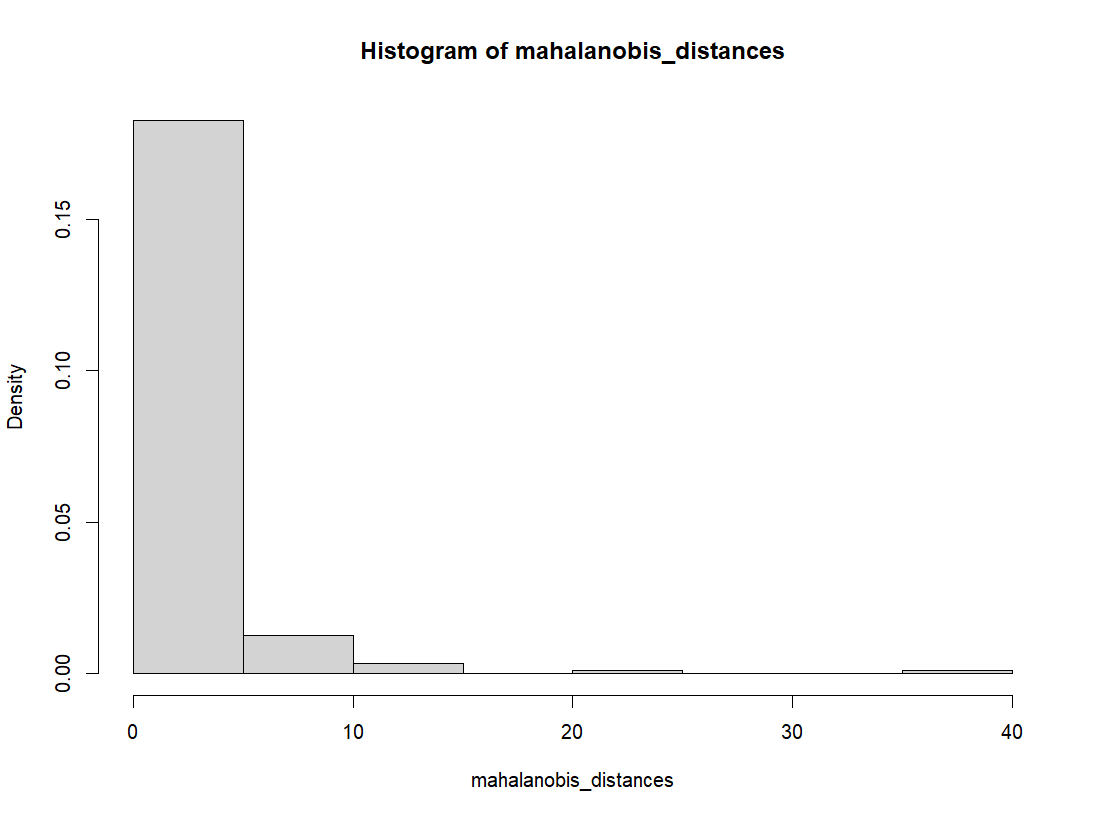
\includegraphics[width=\linewidth]{images/mahalanobis_hist.png}
        \caption{Histogram kwadratów odległości Mahalanobisa}
        \label{fig:mahalanobis_hist}
    \end{subfigure}\hfill
    \begin{subfigure}{0.45\textwidth}
        \centering
        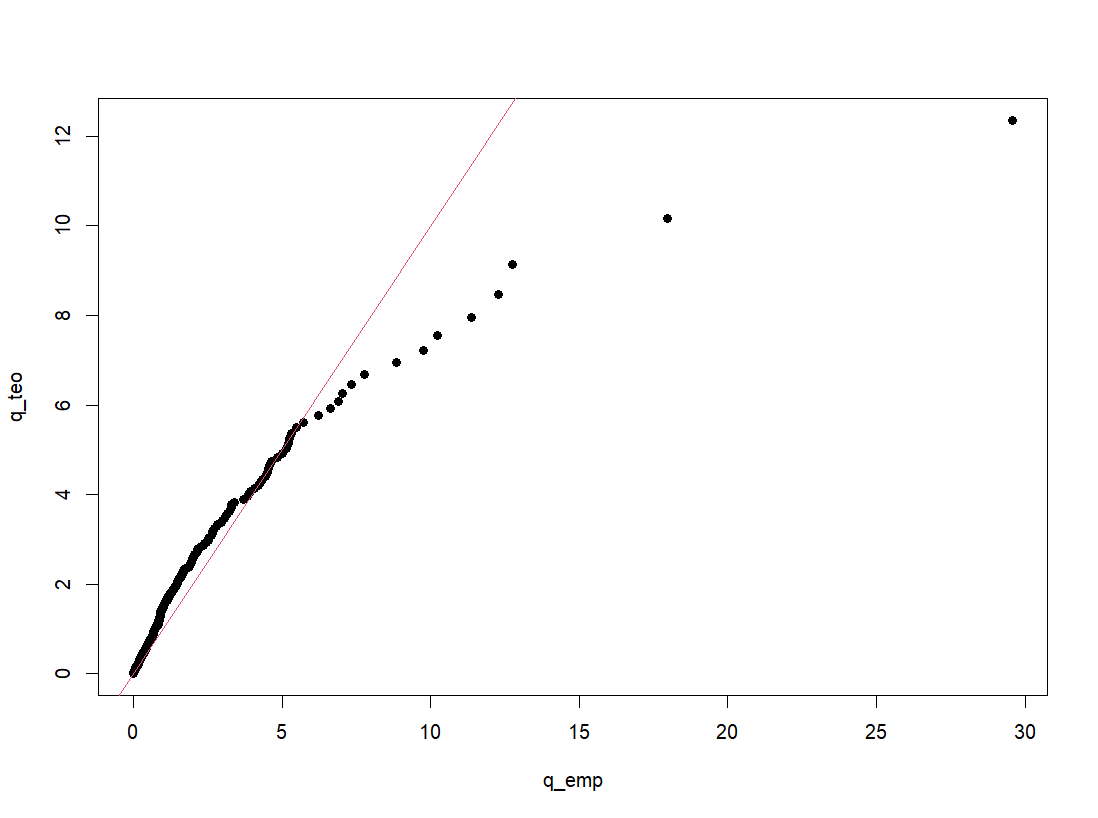
\includegraphics[width=\linewidth]{images/mahalanobis_qqplot.png}
        \caption{QQplot kwantyli empirycznych oraz z rozkładu $\chi^2$}
        \label{fig:mahalanobis_qqplot}
    \end{subfigure}   
    \caption{Analiza odległości Mahalanobisa}
\end{figure}

Punkty w miarę układają się blizko prostej $y = x$ co wskazuje, że rozkład kwadratów odległości Mahalanobisa może być z rozkładu $ \chi^2$

\\
Żeby bardziej się upewnić przeprowadzono test zgodnosci oparty na statystyce Kolmogorova-Smirnova. Wynik testu $p-value = 0.0001707 < 5\%$ zatem odrzucono hipotezę, ze kwadraty odleglości Mahalanobisa mają rozkład $ \chi^2$, co skutkuje też odrzuceniem hipotezy o normalnosci rozkładu log-zwrotow

\section{Regresja liniowa dla log-zwrotów}
\subsection{Wyznaczenie prostej regresji}

Wyznaczono prostą regresji $R_{2} = b_{0} + b_{1} \cdot R_{1}$, (gdzie $R_2$ to spółka JJB, a $R_1$ spółka KMR) zamieszczenie tej prostej na wykresie rozrzutu log-zwrotów można widzieć na rysunku  \ref{fig:linia_regresji}

\begin{figure}[!htb]
	\centering
	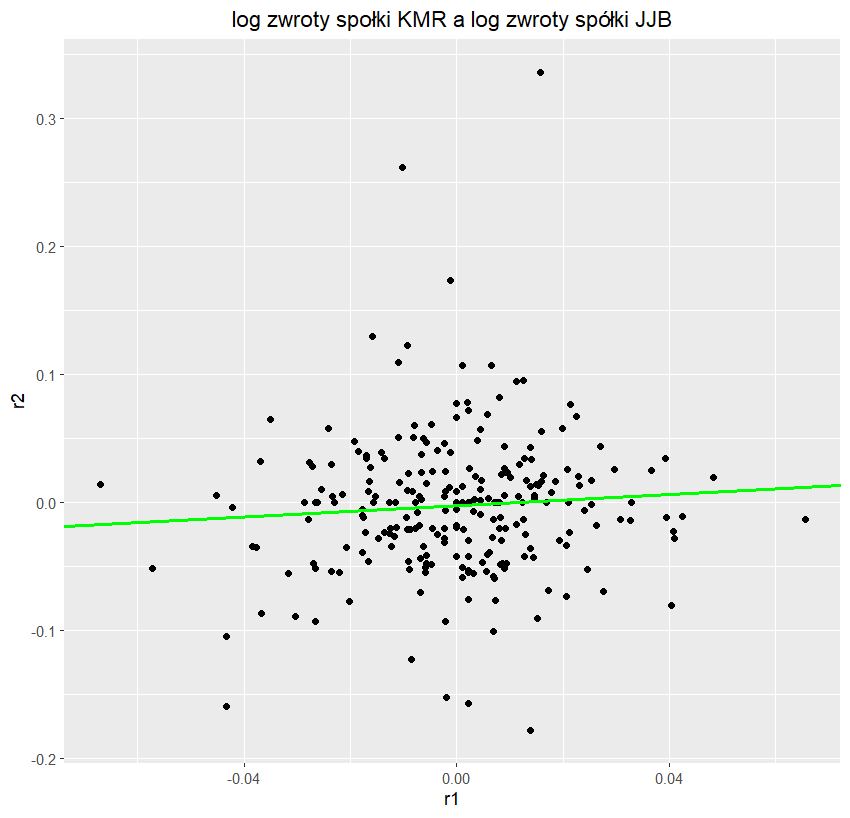
\includegraphics[width=5cm]{images/linia_regresji.png}
	\caption{Linia regresji }
         \label{fig:linia_regresji}
\end{figure}

Wykorzystano model $R_{2} = b_{0} + b_{1} \cdot R_{1} + \epsilon $, zakłądając że $\epsilon \sim N(0, \sigma^2)$. Wyestymowano współczynniki $b_{0}, b_{1}$ metodą najmnijeszych kwadratów, otrzymano $\beta_{1} = 0.2187108, \beta_{0}=-0.002444519$. Skąd linia regresji to $y = -0.0024 + 0.22\cdot x$.

Zrobiona klasyczna regresja w R za pomocą funkcji $lm()$. Otrzymane wyniki można obejrzeć na rysunku \ref{fig:regresja}

\begin{figure}[!htb]
	\centering
	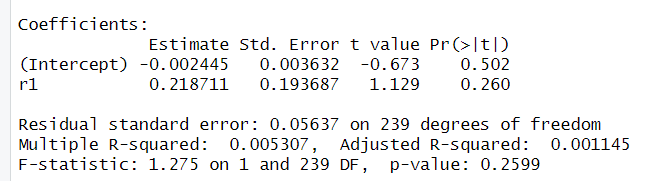
\includegraphics[width=10cm]{images/regresja.png}
	\caption{Wyniki regresji}
         \label{fig:regresja}
\end{figure}

\textbf{Opis otrzymanych wyników modelu regresji}
\begin{enumerate}
  \item (Estimate) są to współczyniki $\hat{b_{0}}=\beta_{0}, \hat{b_{1}}=\beta_{1}$ opisujące linię regresji ($\hat{b_{0}}=-0.002445, \hat{b_{1}}=0.218711$)
  \item  (Residual standard error) Błąd standardowy reszt modelu $\hat{\sigma}$ ($\hat{\sigma} = 0.05637$)
  \item (Multiple R-squared) Współczynnik determinacji R ($R=0.005307$)
  \item (t value, Pr (> |t|)) Wynik testu na istotność współczynników $b_{0}, b_{1}$ – wartość statystyki testowej oraz p-value
  \item (F-statistic) Wynik dodatkowego testu na istotność współczynnika $b_1$

\end{enumerate}

\textbf{Analiza reszt modelu}

Przeprowadzono również analizę reszt modelu, zakładając rozkład normalny $\epsilon \sim N(0, \sigma^2)$. W rozważanym przykłądzie błędem standardowym reszt jest $\hat{\sigma} = 0.05637$. Dlatego analizowano rozkłąd $\epsilon \sim N(0, 0.05637^2)$

Histogram reszt zamieszczono niżej, rysunek \ref{fig:hist_reszty}
\begin{figure}
  \begin{subfigure}{0.5\textwidth}
    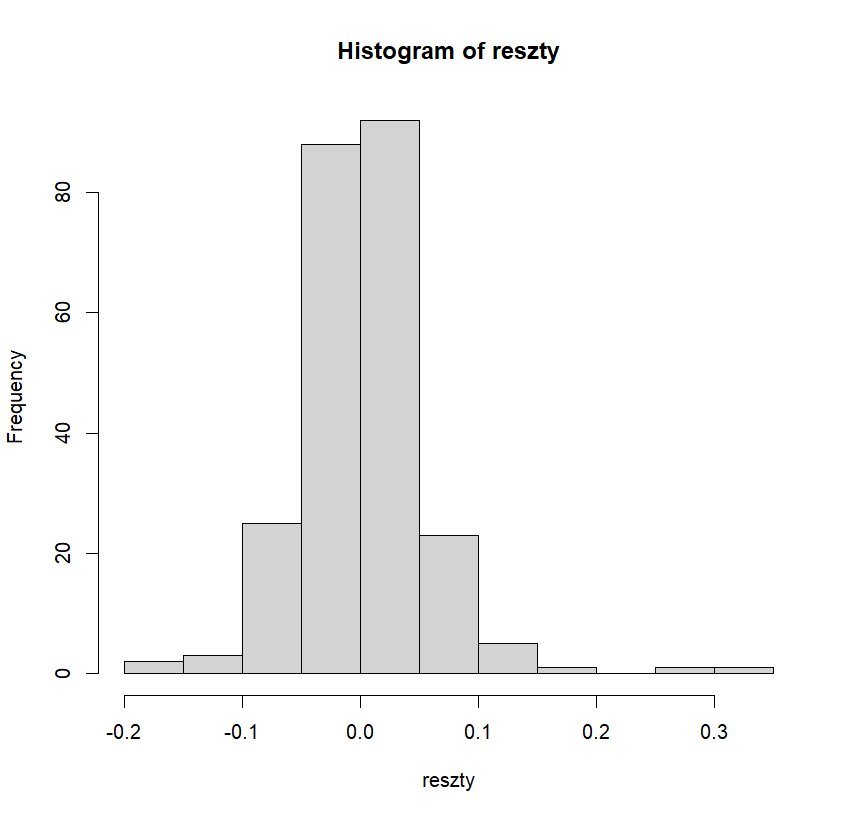
\includegraphics[width=8cm]{images/hist_reszty.png}
    \caption{Histogram reszt regresji}
    \label{fig:hist_reszty}
  \end{subfigure}%
  \begin{subfigure}{0.5\textwidth}
    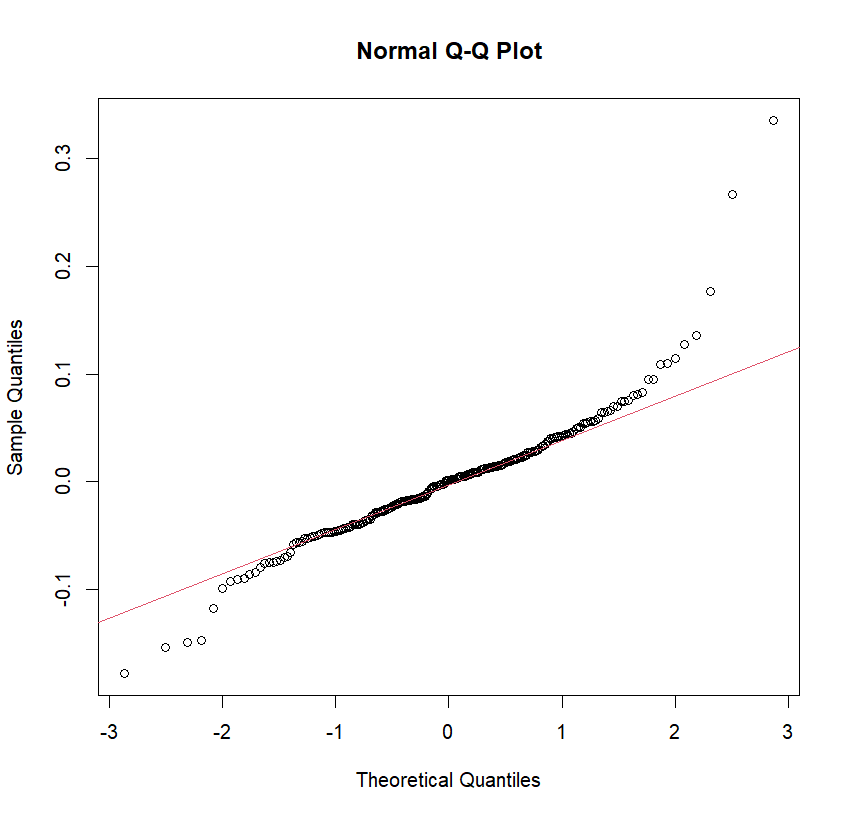
\includegraphics[width=8cm]{images/qq_reszty.png}
    \caption{Wykres diagnostyczny qq-plot reszt}
    \label{fig:qq_reszty}
  \end{subfigure}
  \caption{Analiza reszt modelu regresji}
\end{figure}

Zrobiono wykres diagnostyczny qq-plot dla reszt (rysunek \ref{fig:qq_reszty}), czyli wykres porównujący kwantyle empiryczne oraz teoretyczne. Przy dobrze dopasowanym rozkładzie kwantyle muszą układać się obok prostej $y=x$. Analizując wykres qq-plot, widać że kwantyle układają się w miare obok prostej $y=x$, co wskazuje że rozkład reszt może być rozkładem normalnym $\epsilon \sim N(0, 0.05637^2)$

W celu badania normalności rozkładu reszt wykorzystano metodę Monte Carlo wraz ze statystyką Kołmogorowa-Smirnowa, statystykę Andersona-Darlinga oraz test Shapiro-Wilka. Wartości p-value dla każdego z tych testów umieszczono w tabeli \ref{tab:pvalue}. Ponieważ każda ze statystyk wynosi mniej niż przyjęty poziom istotności 5\%, hipotezę o normalności rozkładu reszt odrzucono



\begin{table}
  \centering
  \begin{tabular}{|c|c|c|} 
   \hline
     KS & AD &Shapiro-Wilk \\
    \hline
    0.04645 & 4.617e-08 & 9.376e-11 \\
    \hline
  \end{tabular}
  \caption{Wartości p-value statystyk}
  \label{tab:pvalue}
\end{table}

\\
\textbf{Współczynnik determinacji R}

Współczynnik determinacji jest jedną z miar jakości dopasowania modelu. Informuje jaka część zmienności zmiennej $r_{2}$ pokrywa się z korelacjami ze zmiennych zawartych w rozważanym modelu. W rozważanym przykładzie $R=0.005307$ oznacza słabe wyjaśnienie zmienności dannych. Mając R=0.5\% wynika że 95\% danych log-zwrotów spółki JJB nie są wyjaśnione przez log-zwroty spółki KMR, można więc rozważyć dodanie do modelu innych zmiennych oprócz log-zwrotów spółki KMR

\\
\textbf{Istotnośc współczynników regresji}

Testowana istotność współczynników regresji $b_{0}$, $b_{1}$, czyli dwie hipotezy ($i = 0, 1$) $H_{0}:\nobreakspace b_{i} = 0 $ przeciwko $H_{1}: b_{i} \ne 0$

Statystyką testową jest \[ t_i = \frac{b_i - \beta_i}{\text{se}(\beta_i)}, i = 0, 1 \] gdzie wielkości $se(\beta_{i})$ to błędy standardowe estymatorów
Jeśli hipoteza zerowa jest prawdziwa, statystyka $T$ ma rozkład t-Studenta o $n-2=241-2=239$ stopniach swobody. Wykres tego rozkładu t-Studenta zamieszczono niżej (rysunek \ref{fig:tStudent})

\begin{enumerate}
  \item Zrobiona hipoteza zerowa $H_{0}$\: $b_{0}=0$ przeciwko hipotezie alternatywnej $H_{1}$: $b_{0} \ne 0$
  Podstawiając dane w powyższy wzór otrzymano: \[ t_0 = \frac{-0.002444519}{0.003632} \approx -0.673\]  

  Otrzymano wyniki $t-value = -0.673$, oraz $Pr(>|t|) = 0.502$. Wartość testu $t_0$ zamiszczono na wykresie kolorem niebieskim. Ponieważ $Pr(>|t|) = 0.502 > 5\%$ hipotezę, że współczynnik $b_{0}$ może być nieistotny przyjęto

  
  
  \item  Zrobiona hipoteza zerowa $H_{0}^{\prime}$: $b_{1}=0$ przeciwko hipotezie alternatywnej $H_{1}^{\prime}$: $b_{1} \ne 0$

  Analogiczno dla wspołczynnika $b_{1}$ podstawiając dane w powyższy wzór otrzymano: \[ t_1 = \frac{0.2187108}{0.193687} \approx 1.129\]  

  Otrzymano wyniki $t-value = 1.129$, oraz $Pr(>|t|) = 0.260$. Wartość testu $t_1$ zamiszczono na wykresie kolorem zielonym. Ponieważ $Pr(>|t|) = 0.260 > 5\%$ hipotezę, że współczynnik $b_{1}$ może być nieistotny przyjęto

\end{enumerate}


\begin{figure}[!htb]
	\centering
	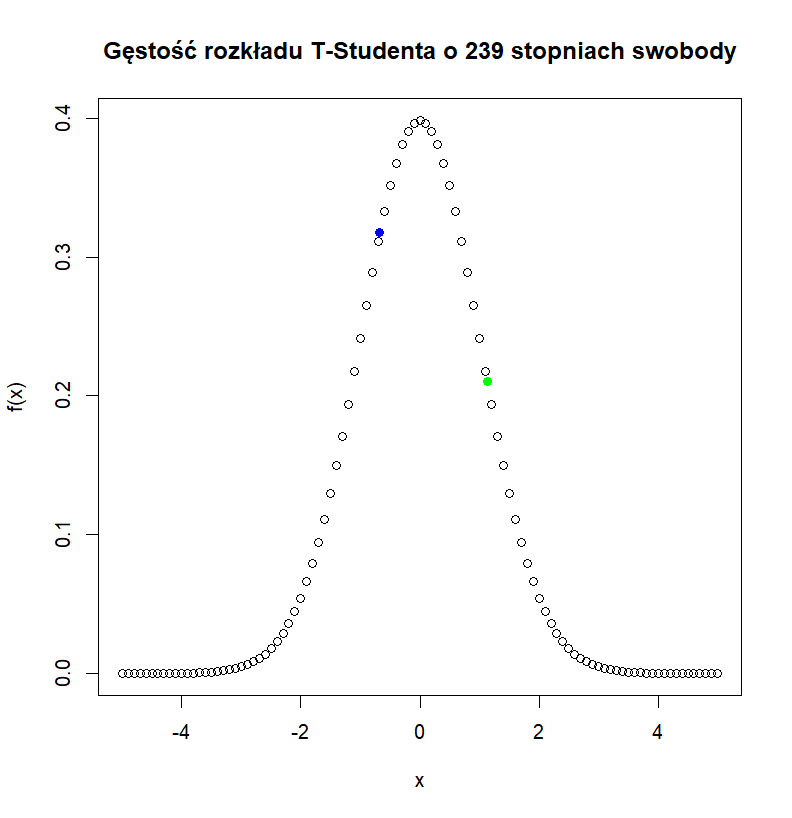
\includegraphics[width=10cm]{images/tStudent.png}
	\caption{Wykres rozkładu t-Studenta}
         \label{fig:tStudent}
\end{figure}

\subsection{Regresja dla uproszczonego modelu}
Ponieważ okazało się, że każdy ze współczynników $b_{0}, b_{1}$ może być nieistotny, wykonano 2 regresji dla uproszczonych modeli

\begin{figure}
  \begin{subfigure}{0.5\textwidth}
    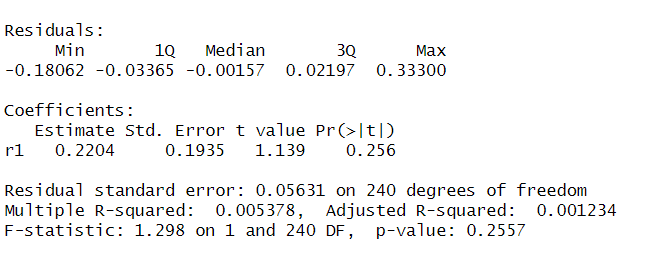
\includegraphics[width=8cm]{images/regresja_upr1.png}
    \caption{Wyniki regresji dla uproszczoego modelu przy $b_{0}=0$}
    \label{fig:regresja_upr1}
  \end{subfigure}%
  \begin{subfigure}{0.5\textwidth}
    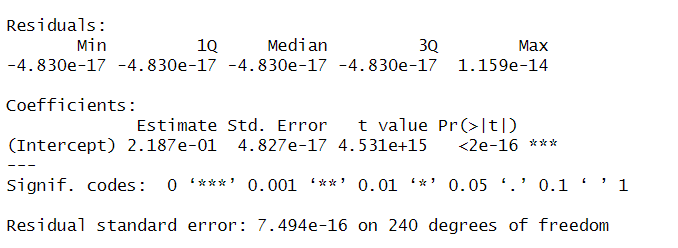
\includegraphics[width=8cm]{images/regresja_upr2.png}
    \caption{Wyniki regresji dla uproszczoego modelu przy $b_{1}=0$}
    \label{fig:regresja_upr2}
  \end{subfigure}
  \caption{Wyniki regresji dla uproszczonych modeli}
\end{figure}


\subsubsection{Uproszczony model przy założeniu $b_{0}=0$}

Przy założeniu $b_{0}=0$, otrzymano model regresji $y=b_{1}\cdot x = 0.22\cdot x$. Wyniki regresji można zobaczyć na rysunku \ref{fig:regresja_upr1}

Duża wartość $Pr(>|t|) = 0.256 > 5\%$ wskazuje, że zostawiony współczynnik może być nieistotny. Współczynnik determinacji $R=0.05631$ wskazuje, że zmienność jest niewyjaśniona tylko zmienną $r_{1}$

\subsubsection{Uproszczony model przy założeniu $b_{1}=0$}

Przy założeniu $b_{1}=0$, otrzymano model regresji $y=b_{0}= -0.0024$. Wyniki regresji można zobaczyć na rysunku \ref{fig:regresja_upr2}

Mała wartość $Pr(>|t|) = <2e^-16 < 5\%$ wskazuje, że zostawiony współczynnik jest istotnym. Współczynnik determinacji $R= 7.494e^-16$ wskazuje, że zmienność jest niewyjaśniona tylko stałą $b_{0}$

\subsection{Predykcja log-zwrotów}
Ponieważ rozważano 3 modeli regresji, zrobiono zostało 3 predykcji wielkości log-zwrotów $R_{2}$ gdy $R_{1}$ bedą na poziomie średniej z rozważanej próbki. W tym celu wyliczono średnią wartość log-zwrotów $R_{1}$. W tym przykłądzie wynosi ona $x^*=-0.0002403422$

\begin{enumerate}
  \item Predykcja dla modelu $y = -0.0024 + 0.22\cdot x$
  
  Predykcja $\hat{y}^*$ gdy wartość $x=\hat{x}^*$ to wartość: $\hat{y}^* = \beta_0 + \beta_1x^*$. Podstawiając dane otrzymano  $\hat{y}^* = -0.002497085$. Czyli jeżeli wartość log-zwrotów spółki KMR będzie wynosiła $-0.0002403$ wartość log-zwrotów spółki JJB będzie wynosiła $-0.002497085$
  
  \item Predykcja dla modelu $y =  0.22\cdot x$
  
   Predykcja $\hat{y}^*$ gdy wartość $x=\hat{x}^*$ to wartość: $\hat{y}^* =\beta_1x^*$. Podstawiając dane otrzymano  $\hat{y}^* = -5.256543e-05$
  \item Predykcja dla modelu $y = -0.0024 $. Czyli jeżeli wartość log-zwrotów spółki KMR będzie wynosiła $-0.0002403$ wartość log-zwrotów spółki JJB będzie wynosiła $-5.256543e-05$

  Predykcja $\hat{y}^*$ gdy wartość $x=\hat{x}^*$ to wartość: $\hat{y}^* = \beta_0 $. Podstawiając dane otrzymano  $\hat{y}^* = -0.002444519$. Czyli jeżeli wartość log-zwrotów spółki KMR będzie wynosiła $-0.0002403$ wartość log-zwrotów spółki JJB będzie wynosiła $-0.002444519$
\end{enumerate}


\section{Podsumowanie}

W projekcie została przeprowadzona analiza cen spółek KMR oraz JJB. Wyliczono statystyki opisowe, wyestymowano parametry rozkładów za pomocą funkcji w języku \textit{R} z biblioteki \textit{fitdistrplus}. Na podstawie analizy wykresów diagnostycznych CDF oraz qqplot, statystyk KS, CM, AD oraz kryteriów informacyjnych AIC, BIC dla każdej ze spółek wybrano najlepsze wykresy. Dla spółki KMR to jest rozkład $LN(6.09, 0.059)$. Dla spółki JJB rozkład $LN(0.67, 0.23)$. Dalej przeprowadzono testowanie hipotez tych rozkładów metodą Monte-Carlo za pomocą statystyki Kolmogorova-Smirnova. W wyniku tego testowania hipotezy o rozkładach logarytmiczno-normalnych spółek nie odrzucone.

W drugiej części projektu badano łączny rozkład log-zwrotów. W celu tej analizy w języku \textit{R} wykorzystano biblioteki \textit{mvtnorm} oraz \textit{MASS}. Na podstawie wykresu rozrzutu zrobiona została hipoteza, że rozkład jest dwuwymiarowy normalny \\ $(X, Y) \sim N(-0.00024, -0.002497, 0.0188, 0.0564, 0.0728)$. Żeby się upewnić w prawdziwości tej hipotezy analizowano również kwadraty odległości Mahalanobisa. Po przeprowadzeniu tej analizy hipotezę o normalności rozkładu log-zwrotów

W trzeciej części projektu wykonano regresję dla rozkładu log-zwrotów. Na podstawie regresji zrobiona predykcja wartości log-zwrotów spółki KMR jeżeli wartość log-zwrotów spółki będą na poziomie średniej. Otrzymano wynik: jeżeli wartość log-zwrotów spółki KMR będzie wynosiła $-0.0002403$ wartość log-zwrotów spółki JJB będzie wynosiła $-0.002$


\end{document}